\section{State estimation}

To validate the algorithm, three sets of data that had good information from the cars Dual-\gls{GPS} was found. Two sets are from the actual dynamic event called "Endurance" during the two competition \gls{FSS} and \gls{FSG}. These two data sets are called "FSS Endurance" and "FSG Endurance", respectively. The last data set is from a test track at \gls{FSG} that the team had access to in the days before the competition started, called "FSG Test Track 1". 

The RTK-GPS data were all corrupted by sporadic outliers, so a preprocessing step to remove them was done. A preprocessing step of the yaw angle data was also needed, since the internal Kalman filter of the \gls{INS} restricted the yaw to the interval $[-\pi,\pi]$ radians. 

The data sets all had varying degrees of quality of the ground truth. They did however all suffer more or less the same from one rather large flaw; last years team had not managed to turn on the internal Kalman filtering of the \gls{INS} data. This has been corrected now, but this means that the results shown below are different, and most likely worse, than what is going to be seen when the test period begins.

\subsubsection{Ground truth quality}

The first data set, "FSS Endurance", had no \gls{GPS} position data that was usable, but the longitudinal velocity and yaw rate were both good, as well as the yaw angle. The lateral velocity is usable, but definitely not perfect. This is considering how large the side slip angles are, regularly going up to values of 10-15\si{\degree}, which after discussing with the drivers at the event and the vehicle dynamics group seem unreasonably high. The car is not built to side slip that much at those velocities, nor are the drivers instructed to drive so recklessly, especially not during the endurance event where saving energy is key. 

The results of the state estimator compared to ground truth for longitudinal  and lateral velocity, yaw rate and yaw angle on the "FSS Endurance" is seen in figures \ref{Fig:VxFSSEndurance}, \ref{Fig:VyFSSEndurance}, \ref{Fig:RFSSEndurance}, \ref{Fig:YawFSSEndurance}, respectively. The integrated position without ground truth is shown in \ref{Fig:PosFSSEndurance}. 

The second data set, "FSG Endurance", had good position data, as well as good longitudinal velocity and yaw angle. The lateral velocity and yaw rate were however not good enough to use for comparison. The results compared with ground truth for this data set is shown in \ref{Fig:PosFSGEndurance}, \ref{Fig:YawFSGEndurance} and \ref{Fig:VxFSGEndurance}. 

The last data set, "FSG Test Track 1", like data set "FSS Endurance", had no usable position data, but the longitudinal velocity, yaw rate and yaw angle were all good. The lateral velocity is okay, at least we do not have any reason to not trust it, as it was a really short track with a lot of turning, and the data seems to fit with the way they would have driven it and the way the car was expected to behave. 

The results of the state estimator compared to ground truth for longitudinal  and lateral velocity, yaw rate and yaw angle on the "FSG Test Track 1" is seen in figures \ref{Fig:VxFSGTestTrack}, \ref{Fig:VyFSGTestTrack}, \ref{Fig:RFSGTestTrack}, \ref{Fig:YawFSGTestTrack}, respectively. The integrated position without ground truth is shown in \ref{Fig:PosFSGTestTrack}. 

\subsubsection{Overall results}

The results obtained so far show low error on the longitudinal velocity and yaw rate and seems to give good position estimates. The lateral velocity on the other hand is more uncertain. It does not match perfectly the ground truth. This might be because of poor ground truth data. Either way the lateral velocity is not the most important, as long as the overall pose estimate has low drift. 

\FloatBarrier

% FSS Endurance
\begin{figure}
    \centering
    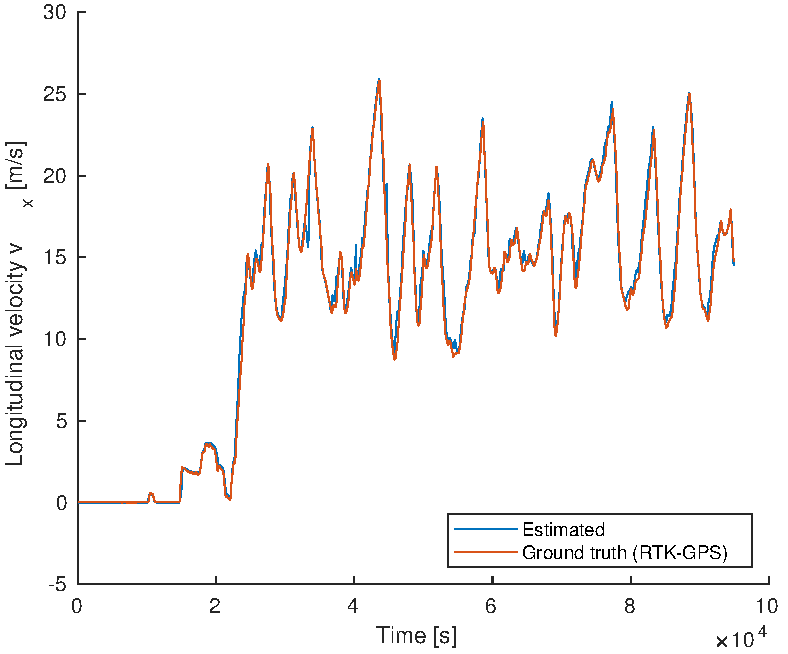
\includegraphics[width=0.8\linewidth]{0_Images/6_Results/vxFSSEndurance.pdf}
    \caption[Longitudinal velocity while driving FSS Endurance.]
    {Longitudinal velocity  while driving FSS Endurance. Estimated compared with data from the INS.}
    \label{Fig:VxFSSEndurance}
\end{figure}
\begin{figure}
    \centering
    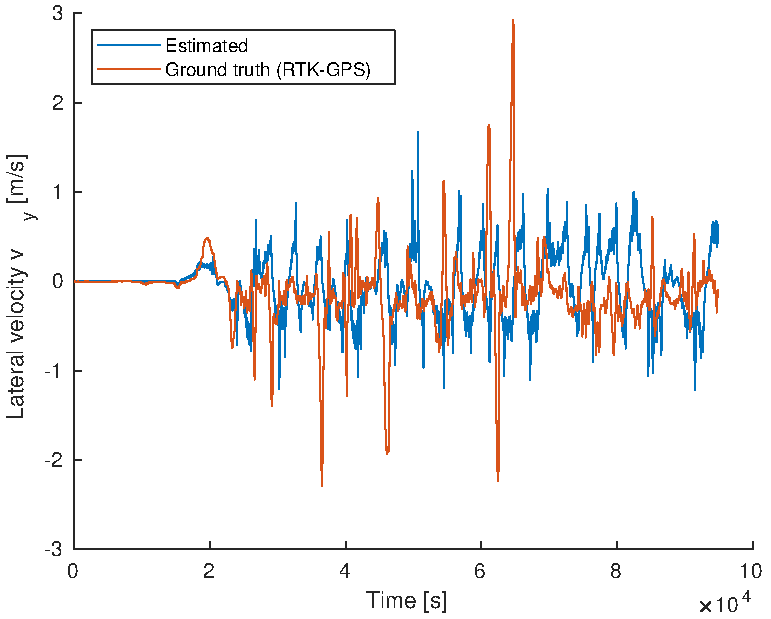
\includegraphics[width=0.8\linewidth]{0_Images/6_Results/vyFSSEndurance.pdf}
    \caption[Lateral velocity while driving FSS Endurance.]
    {Lateral velocity while driving FSS Endurance. Estimated compared with data from the INS.}
    \label{Fig:VyFSSEndurance}
\end{figure}

\begin{figure}
    \centering
    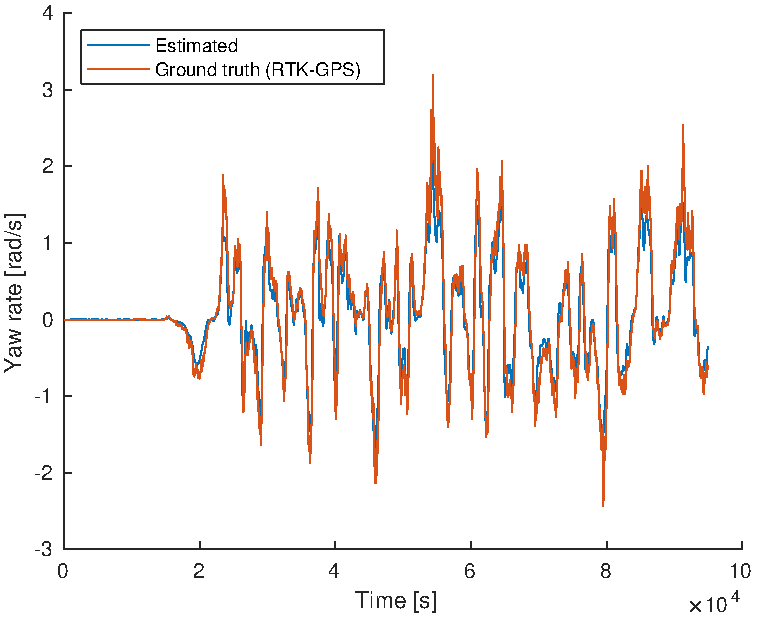
\includegraphics[width=0.8\linewidth]{0_Images/6_Results/rFSSEndurance.pdf}
    \caption[Yaw rate while driving FSS Endurance.]
    {Yaw rate  while driving FSS Endurance. Estimated compared with data from the INS.}
    \label{Fig:RFSSEndurance}
\end{figure}

\begin{figure}
    \centering
    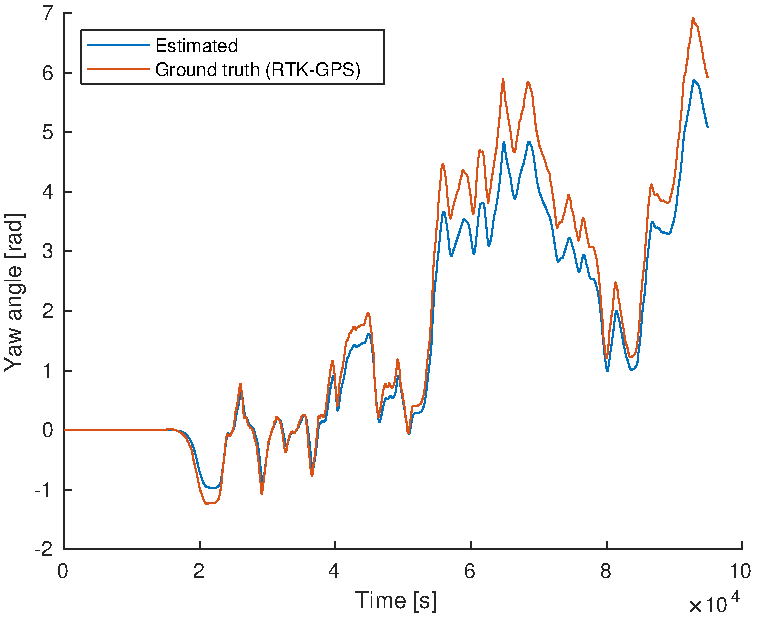
\includegraphics[width=0.8\linewidth]{0_Images/6_Results/yawFSSEndurance.pdf}
    \caption[Yaw angle while driving FSS Endurance.]
    {Yaw angle while driving FSS Endurance. Estimated compared with data from the INS.}
    \label{Fig:YawFSSEndurance}
\end{figure}

\begin{figure}
    \centering
    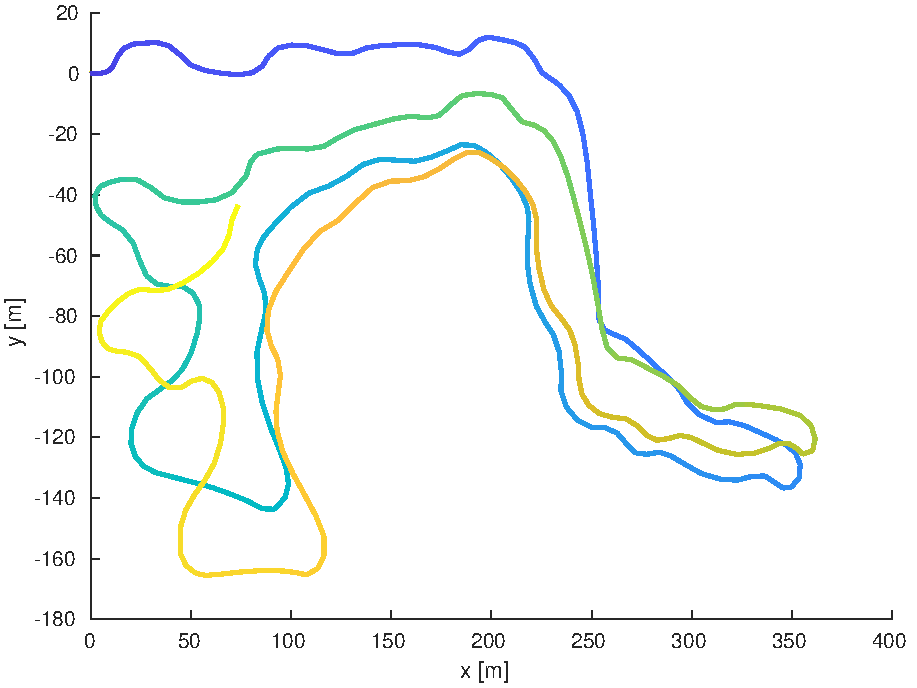
\includegraphics[width=0.8\linewidth]{0_Images/6_Results/positionFSSEndurance.pdf}
    \caption[Position while driving FSS Endurance.]
    {Position while driving FSS Endurance.}
    \label{Fig:PosFSSEndurance}
\end{figure}


%% FSG Endurance

\begin{figure}
    \centering
    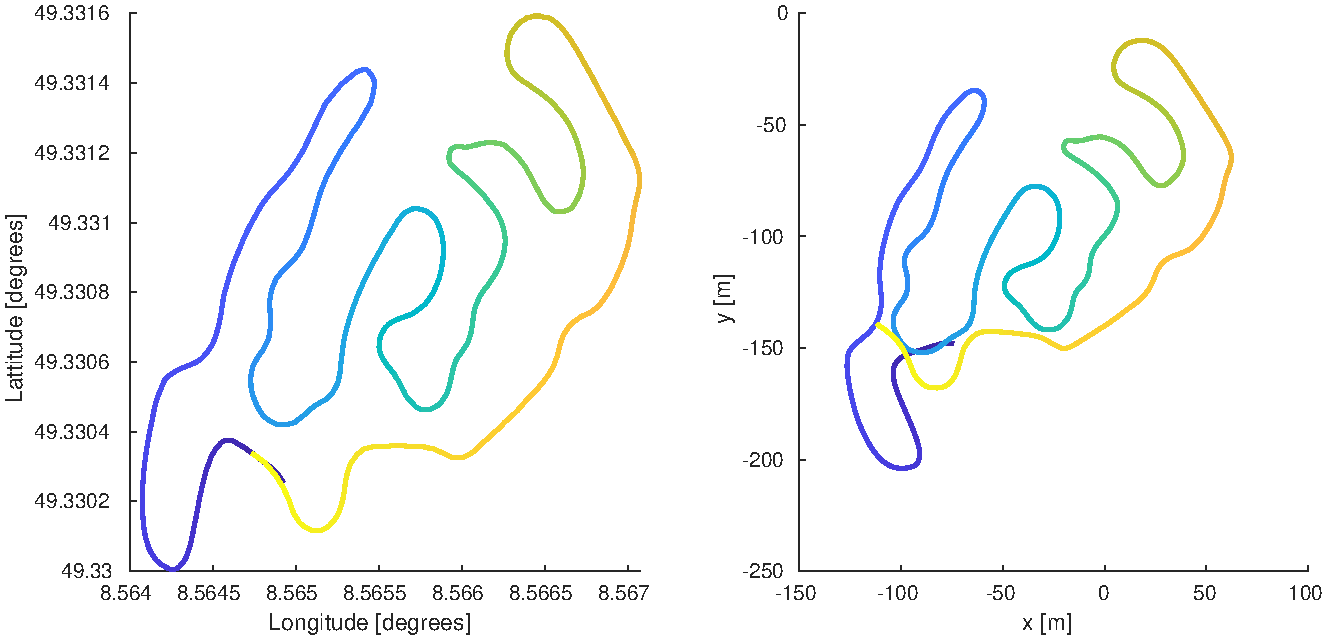
\includegraphics[width=0.8\linewidth]{0_Images/6_Results/positionFSGEndurance.pdf}
    \caption[Position while driving FSG Endurance.]
    {Position while driving FSG Endurance. Left is data from the INS while the right is estimated.}
    \label{Fig:PosFSGEndurance}
\end{figure}

\begin{figure}
    \centering
    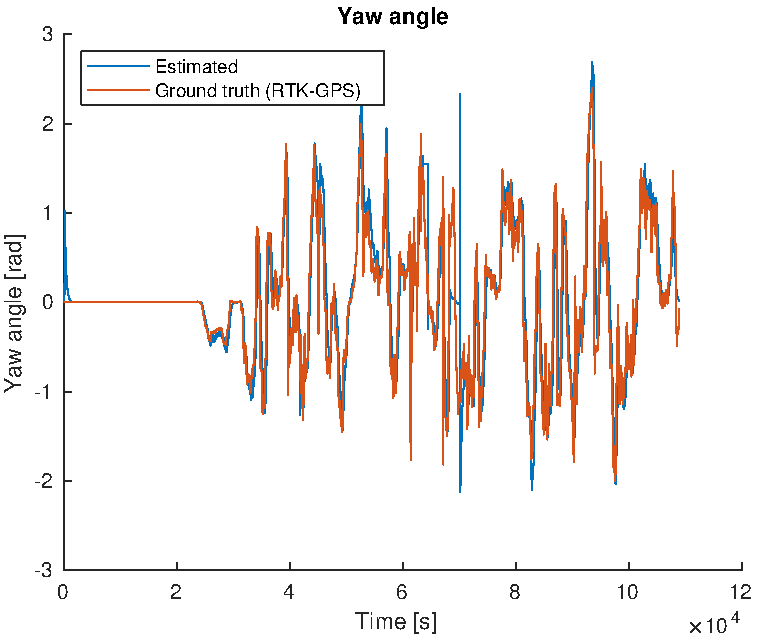
\includegraphics[width=0.8\linewidth]{0_Images/6_Results/yawFSGEndurance.pdf}
    \caption[Yaw angle while driving FSG Endurance.]
    {Yaw angle while driving FSG Endurance. Estimated compared with data from the INS.}
    \label{Fig:YawFSGEndurance}
\end{figure}

\begin{figure}
    \centering
    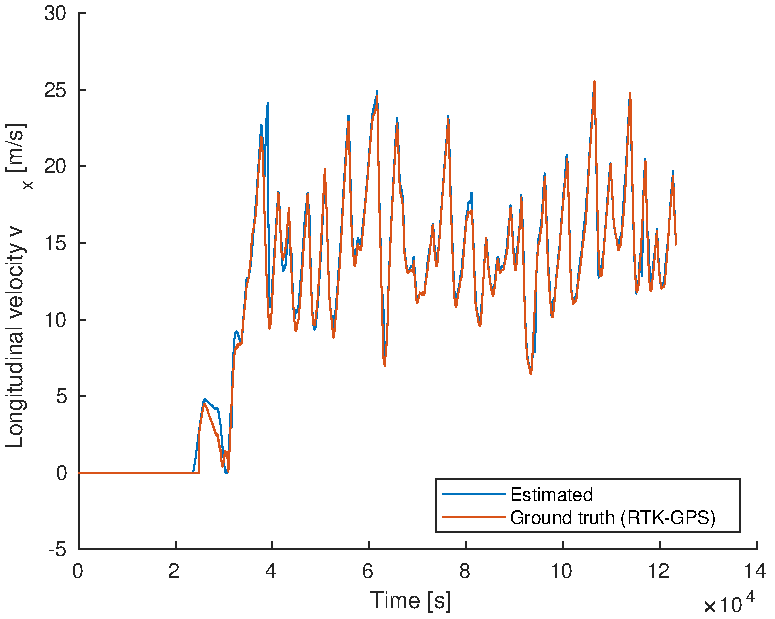
\includegraphics[width=0.8\linewidth]{0_Images/6_Results/vxFSGEndurance.pdf}
    \caption[Longitudinal velocity while driving FSG Endurance.]
    {Longitudinal while driving  during FSG Endurance. Estimated compared with data from the INS.}
    \label{Fig:VxFSGEndurance}
\end{figure}

%% FSG Test track 1

\begin{figure}
    \centering
    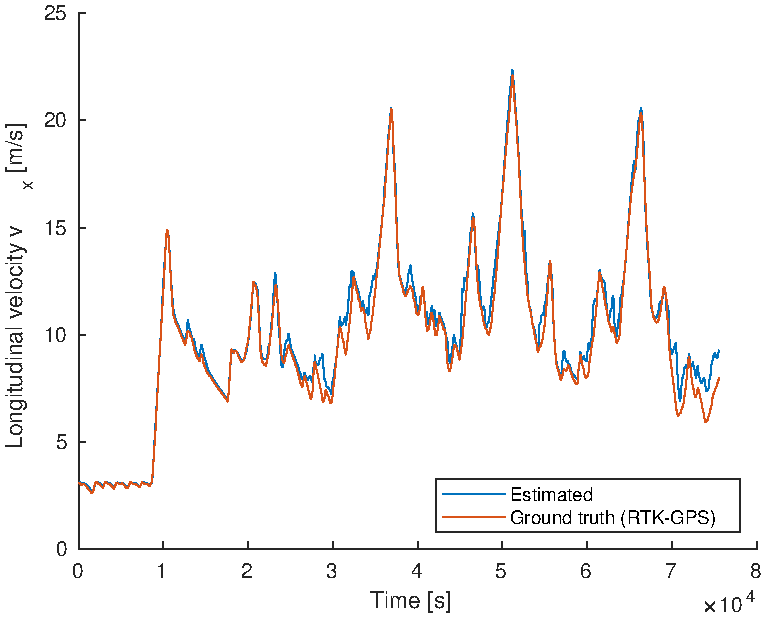
\includegraphics[width=0.8\linewidth]{0_Images/6_Results/vxFSGTestTrack.pdf}
    \caption[Longitudinal velocity while driving FSG Test Track 1.]
    {Longitudinal velocity while driving FSG Test Track 1. Estimated compared with data from the INS.}
    \label{Fig:VxFSGTestTrack}
\end{figure}

\begin{figure}
    \centering
    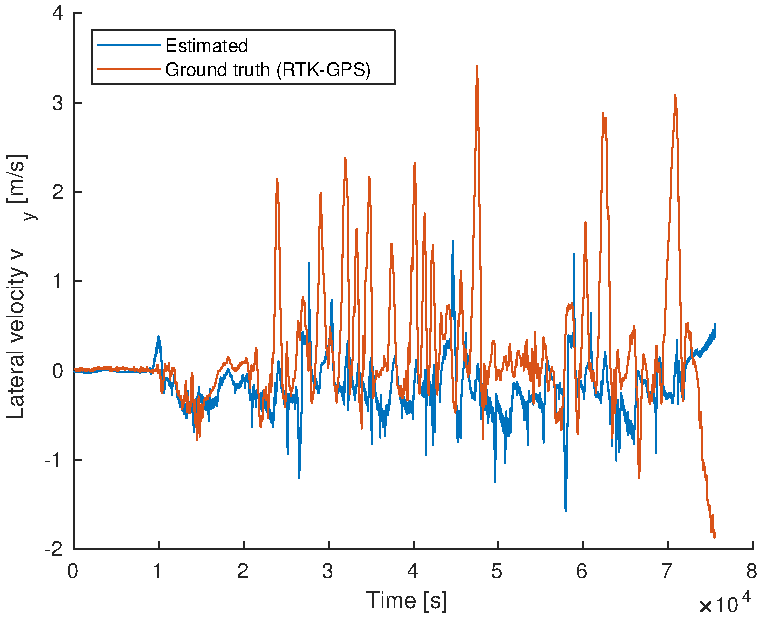
\includegraphics[width=0.8\linewidth]{0_Images/6_Results/vyFSGTestTrack.pdf}
    \caption[Lateral velocity while driving FSG Test Track 1.]
    {Lateral velocity  while driving FSG Test Track 1. Estimated compared with data from the INS.}
    \label{Fig:VyFSGTestTrack}
\end{figure}

\begin{figure}
    \centering
    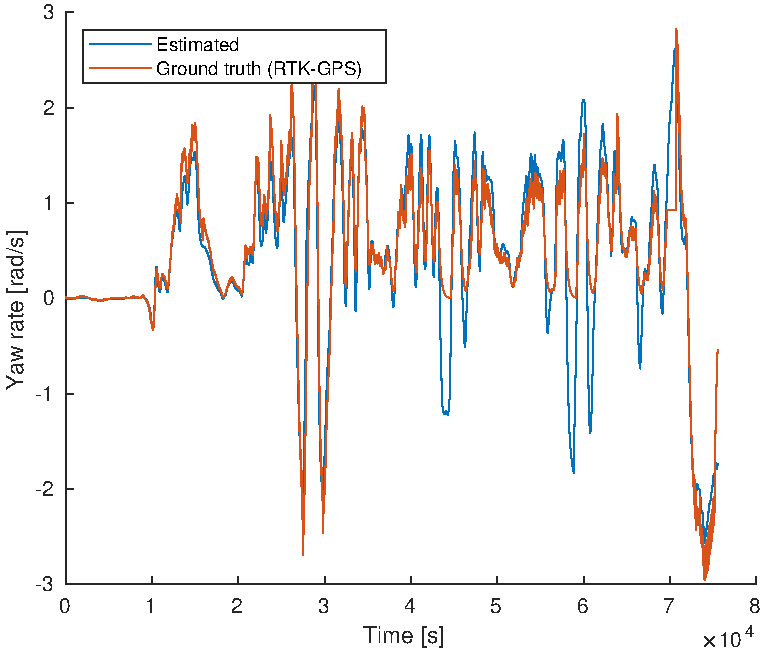
\includegraphics[width=0.8\linewidth]{0_Images/6_Results/rFSGTestTrack.pdf}
    \caption[Yaw rate while driving FSG Test Track 1.]
    {Yaw rate while driving FSG Test Track 1. Estimated compared with data from the INS.}
    \label{Fig:RFSGTestTrack}
\end{figure}

\begin{figure}
    \centering
    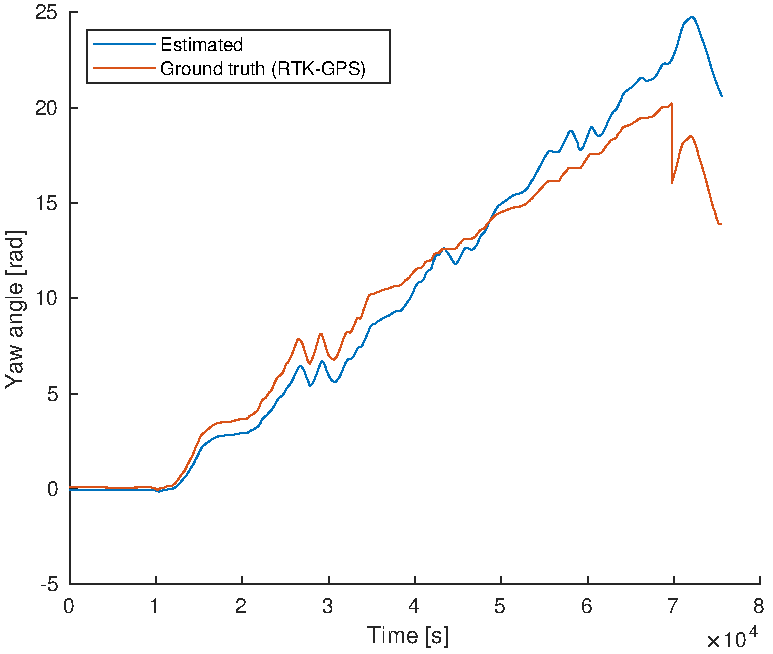
\includegraphics[width=0.8\linewidth]{0_Images/6_Results/yawFSGTestTrack.pdf}
    \caption[Yaw angle while driving FSG Test Track 1.]
    {Yaw angle while driving FSG Test Track 1. Estimated compared with data from the INS.}
    \label{Fig:YawFSGTestTrack}
\end{figure}

\begin{figure}
    \centering
    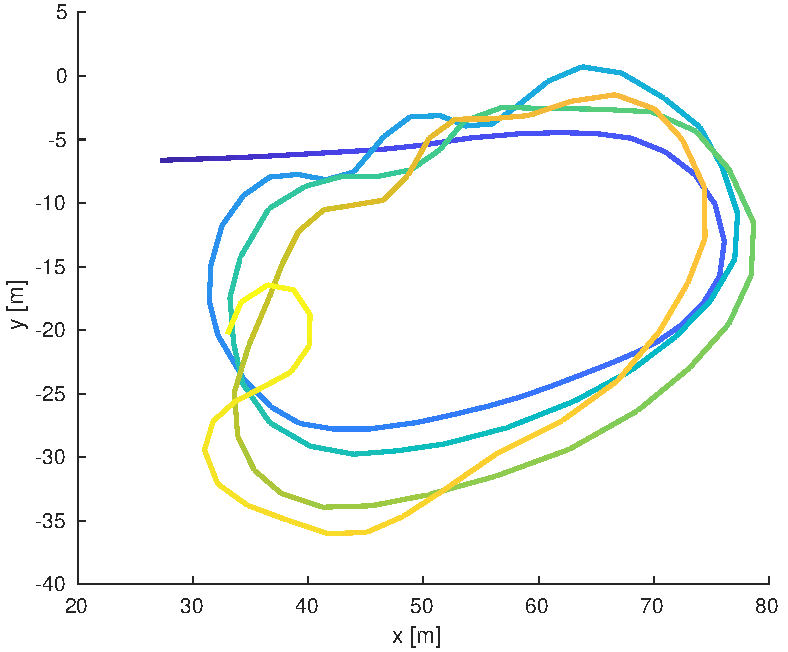
\includegraphics[width=0.8\linewidth]{0_Images/6_Results/positionFSGTestTrack.pdf}
    \caption[Position while driving FSG Test Track 1.]
    {Position while driving FSG Test Track 1.}
    \label{Fig:PosFSGTestTrack}
\end{figure}

\FloatBarrier